% Use only LaTeX2e, calling the article.cls class and 12-point type.

\documentclass[12pt]{article}

\usepackage{amsmath}
\usepackage[normalem]{ulem}
\usepackage{graphicx}

% The following parameters seem to provide a reasonable page setup.
\topmargin 0.0cm
\oddsidemargin 0.2cm
\textwidth 16cm 
\textheight 21cm
\footskip 1.0cm

% Include your paper's title here

\title{Tetrahedral Lagrange Polynomial Interpolation} 
\author{Aleksejs Fomins}
\date{}

%%%%%%%%%%%%%%%%% END OF PREAMBLE %%%%%%%%%%%%%%%%

\begin{document} 

% Double-space the manuscript.
% \baselineskip24pt

% Make the title.
\maketitle 

\section{Polynomial class}

\noindent
Here we discuss the analytical implementation and storage of polynomials for arbitrary dimension and parameter number.

\subsection{Theory}

Arbitrary polynomial of order up to $n$ with $d$ parameters can be represented in its expanded form as
\[ p(\vec{u}) = \sum_i A_i \prod_{j = 0}^d u_j^{\mathrm{pow}_{i,j}},  \]
for example in 3D this can be written as
\[ p(\vec{u}) = \sum_i A_i u^{pow_{u,i}} v^{pow_{v,i}} w^{pow_{w, i}},  \]

\noindent
Therefore, we define a PolySummand class, which stores a constant multiplier $A$ and powers vector $pow$, and Polynomial class
which stores a vector of PolySummands, and does required operations on them. Below we describe the implemented functionality

\subsection{Methods}

\begin{itemize}
	\item \uline{Initialization}: empty or with a single summand
	\item \uline{Operators}: adding, subtracting or multiplying 2 polynomials or polynomial and a scalar.
		\subitem - to multiply by constant, need to loop and multiply each $A_i$ by constant
		\subitem - to add or subtract 2 polynomials, merge the summand vectors and compactify
		\subitem - to multiply 2 polynomials, constructing a new polynomial from pairwise products of all summands, and compactify
	\item \uline{Evaluate}: evaluates all summand and adds them up.
	\item \uline{Take derivative}: lowers the corresponding power for each summand, multiplies prefactor by that power, and removes the summands that differentiate to 0
	\item \uline{Compactify}: adds up all summands with the same power. Sorts the summands by $(x_1,y_1,z_1) < (x_2, y_2, z_2)$, where $x$ has the highest priority and $z$ has the lowest priority. Then all of the repeating powers will be consecutive. Simply loop over sorted polynomial, and to a new polynomial add the sums of all consecutive repeating polynomials.
	\item \uline{Integrate}: Integration of a polynomial over a reference simplex. Naturally, it is the sum of integrals of summands. It can be shown that
		\subitem - 1D integral over the reference edge is $A \frac{1}{pow_u + 1}$
		\subitem - 2D integral over the reference triangle is $A \frac{pow_u! pow_v!}{(pow_u + pow_v + 2)!}$
		\subitem - 3D integral over the reference tetrahedron is $A \frac{pow_u! pow_v! pow_w!}{(pow_u + pow_v + pow_w + 3)!}$
\end{itemize}

\subsection{Tests}

\noindent
Currently the tests are only for 1, 2 and 3 dimensions. Most of the tests use intrinsic functionality like polynomial operators and derivatives to construct polynomials and print them to the screen, and request the user to to verify manually if they match the expected polynomials which are also printed. For each dimension there is one test which integrates a non-linear polynomial over simplex and prints out the result which is also compared manually. \\

\textbf{TODO:} These tests can and should be automatized in the future using integer string comparison. The test program should throw an error if a test fails



\section{Curvilinear Element Interpolation class}

\noindent
Here we describe how to construct a curvilinear 3D object (edge, triangle or tetrahedron) which is interpolated over a set of points. \\

\subsection{Interpolatory Points}

\noindent
We start by assuming a parameterization of the reference entity, namely
\begin{itemize}
	\item edge:			$\vec{r}=(u)$,		such that $u \in [0,1]$
	\item triangle: 	$\vec{r}=(u,v)$,	such that $u \in [0,1]$ and $v \in [0, 1-u]$
	\item tetrahedron:	$\vec{r}=(u,v,w)$,	such that $u \in [0,1]$, $v \in [0, 1-u]$ and $w \in [0, 1-u-v]$ 
\end{itemize}

\noindent
Next, we provide a set of real geometry points $\vec{p}_i(\vec{r}_i)$ over which the 3D object is interpolated. By convention, we choose a rectangular grid in the parametric space, namely providing a real geometry point for each $\vec{r}_{i,j,k} = \Delta (i,j,k)$, where $i,j,k$ are integers, $\Delta = 1 / (Ord - 1)$ is the parametric step size, and $Ord$ is the interpolation order of the surface. The parametric coordinates and their order determine the Lagrange Interpolatory polynomials and must be kept track of. Although the above convention is used in this writeup, the formalism itself can be applied to any set of interpolatory points, as long as their amount is preserved. In particular, for higher orders it should be beneficial to switch to Chebyshev sampling in order to minimize the Runge phenomenon. \\

\noindent
It is easy to verify that the above discretization generates the following number of interpolatory points as a function of interpolatory order (starting with 1, mentioning first 5 orders)
\begin{itemize}
	\item edge:			$N_{Ord} = \{ 2,3,4,5,6 \}  $
	\item face:			$N_{Ord} = \{ 3,6,10,15,21 \}  $
	\item tetrahedron:	$N_{Ord} = \{ 4,10,20,35,56 \}  $
\end{itemize}

\subsection{Interpolatory Polynomials}
\label{section-interppoly}

\noindent
Also, it is easy to verify, that the numbers of interpolatory points above exactly match the numbers of independent polynomials of all orders up to and including $Ord$. Let us define the functions $z^{(1,i)}(u)$, $z^{(2,i)}(u,v)$ and $z^{(3,i)}(u,v,w)$ as the set of all such polynomials, where the first number is dimension of the object, and the 2nd is the order:
\begin{itemize}
	\item edge: \\
		$z^{(1,1)}(u) = \{1, u\}$, \\
		$z^{(1,2)}(u) = \{1, u, u^2\}$, \\
		$z^{(1,3)}(u) = \{1, u, u^2, u^3\}$, \\
		$z^{(1,4)}(u) = \{1, u, u^2, u^3, u^4\}$, \\
		$z^{(1,5)}(u) = \{1, u, u^2, u^3, u^4, u^5\}$, \\
		etc
	\item face:	\\
		$z^{(2,1)}(u,v)	= \{1, u, v\}$, \\
		$z^{(2,2)}(u,v) = \{1, u, v, u^2, uv, v^2\}$, \\
		etc
	\item tetrahedron: \\
		$z^{(2,1)}(u,v,w) = \{1, u, v, w\}$, \\ 
		$z^{(2,2)}(u,v,w) = \{1, u, v, w, u^2, uv, v^2, wu, wv, w^2\}$, \\
		etc
\end{itemize}

\noindent
This means that we are able to use complete polynomials of given order for our interpolation. If one interpolates over other entities, for example, rectangles, one has to either use an incomplete basis of certain order in order to keep the rectangular sampling grid convention, or change the sampling convention to have exact number of interpolatory points for a certain order. $[Volakis2010]$ choose the first approach, thus interpolating a 9 node 2nd order rectangle with 4th order incomplete polynomial which has a convenient separable dimension product form. \\

\noindent
Now, \textbf{the idea of Lagrange Interpolation} is to generate a polynomial vector function $\vec{p}(\vec{r})$, which would correspond to a real point $\vec{p}_i = \vec{p}(\vec{r}_i)$ for each parametric coordinate $\vec{r}_i$ corresponding to a point in the reference element. It can be easily seen that such function must take the form
\begin{equation}
	\vec{p}(\vec{r}) = \sum_j L_j(\vec{r})\vec{p}_j 
\end{equation}
\noindent
where the Lagrange Polynomials $L_j$ are defined by their interpolatory property
\begin{equation}
	\label{equation-lagrangepol-interpolatory-property}
	L_j(\vec{r}_i) = \delta_{ij}
\end{equation}
\noindent
for all interpolatory points $\vec{r}_i$. It is easy to see that in general case there must be as many Lagrange Polynomials as there are interpolatory points $N_{Ord}$, and, the amount of free parameters within each polynomial must also be equal to that number, such that it can uniquely interpolate a set of $N_{Ord}$ points ($N_{Ord} - 1$ zeroes and 1 one). As we have discussed above, this is indeed the case.

\noindent
Next, one slightly tricky part, and then we are done. We would like to prove that the following equation holds:
\begin{equation}
	\label{equation-lagrangepol-basis-link}
	z_i(\vec{r}) = \sum_j L_j(\vec{r}) z_i (\vec{r}_j) 
\end{equation}
\noindent
where $z_i$ is a vector of standard polynomials defined above. This equation should hold for all $z^{(\dim, Ord)}$, where $\dim = \{1,2,3\}$. For $\dim < 3$ where $z$ is defined for less than 3 parameters, simply ignore the extra parameters in $\vec{r}$. \\

\noindent
The proof is quite simple. Both LHS and RHS are polynomials of order at most $Ord$, which means that they have at most $N_{Ord}$ free parameters, and therefore, if we can show that the equation holds for $N_{Ord}$ different parameter sets, then it holds for all others as well. And indeed, \eqref{equation-lagrangepol-basis-link} holds for all $\vec{r} = \vec{r}_k$ because of \eqref{equation-lagrangepol-interpolatory-property}. \\

\noindent
Finally, we can write \eqref{equation-lagrangepol-basis-link} as a vector equation
\begin{equation}
	\vec{z} (\vec{r}) = V \vec{L} (\vec{r})
\end{equation}
\noindent
where $V_{ij} = z_i (\vec{r}_j)$, and find the Lagrange polynomials by inverting $V$, namely
\begin{equation}
	\vec{L} (\vec{r}) = V^{-1} \vec{z} (\vec{r})
\end{equation}
\noindent
Thus each Lagrange Polynomial is a linear combination of standard polynomials. They are polynomials of order (at most) $Ord$. Depending on whether we are dealing with edges, faces or tetrahedrons, $L_j$ will be a function of 1, 2 or 3 parameters.

\subsection{Discussion}

\noindent
Important question is the interpretation of the interpolated manifold
\begin{itemize}
	\item edge: a bounded curve which connects a certain set of points
	\item triangle: a bounded surface which connects a certain set of points
	\item tetrahedron: a bounded volume which connects a certain set of points
\end{itemize}

\noindent
It is important to understand, especially for the tetrahedral case, that the parameterized bounded manifold is not exhaustively defined by the shape of its boundary. In tetrahedral case, interpolation over points associated with the element itself does not only mean that the interpolatory point is located inside of the tetrahedron. What it means that the geometry within the tetrahedron is also curved, such that all points within the parametric reference tetrahedron are uniquely mapped to the points in the real tetrahedron.


\subsection{Implementation for Simplices}
\label{subsection-simplexgrid}

\noindent
In this section we discuss how to efficiently enumerate the simplex interpolatory points, and to construct the reference simplex grid. \\

\noindent
Let us place a set of points $\vec{\eta} \in Z^{\dim}$ over simplex $\Delta^{\dim}_{\mathrm{len}}$. This can be done trivially
by using 3 for loops and pushing vectors into a vector
\begin{itemize}
	\item $\Delta^{1}_n = \{(i)\}$, for $i = [1$ to $n]$
	\item $\Delta^{2}_n = \{(j,i)\}$, for $i = [1$ to $n]$, $j = [1$ to $n - i]$
	\item $\Delta^{3}_n = \{(k,j,i)\}$, for $i = [1$ to $n]$, $j = [1$ to $n - i]$, $k = [1$ to $n - i - j]$
\end{itemize}

\noindent
Then, each point $(\Delta^{d}_n)_i$ corresponds exactly to the power of $u,v,w$ in the expansion of $(1 + u + v + w)^n$, namely
\[ (1 + u)^n = \sum_{i=0}^n C^{(\Delta^{1}_n)_i}_n u^{(\Delta^{1}_n)_{i,1}} \]
\[ (1 + u + v)^n = \sum_{i=0}^n C^{(\Delta^{1}_n)_i}_n u^{(\Delta^{1}_n)_{i,1}} v^{(\Delta^{1}_n)_{i,2}} \]
\[ (1 + u + v + w)^n = \sum_{i=0}^n C^{(\Delta^{1}_n)_i}_n u^{(\Delta^{1}_n)_{i,1}} v^{(\Delta^{1}_n)_{i,2}} w^{(\Delta^{1}_n)_{i,3}} \]

\noindent
where $C^{i}_n, C^{i,j}_n$ and $C^{i,j,k}_n$ are the binomial, trinomial and quatranomial coefficients. The powers of the parameters given in this way are exactly the complete monomial basis for a polynomial of order up to and including $d$. \\

\noindent
Also, it is convenient to note that $(\Delta^{d}_n)_i / n$ is exactly the parametric coordinates of the interpolation points on a regular grid over simplex. 

\begin{figure}[hp]
    \centering
    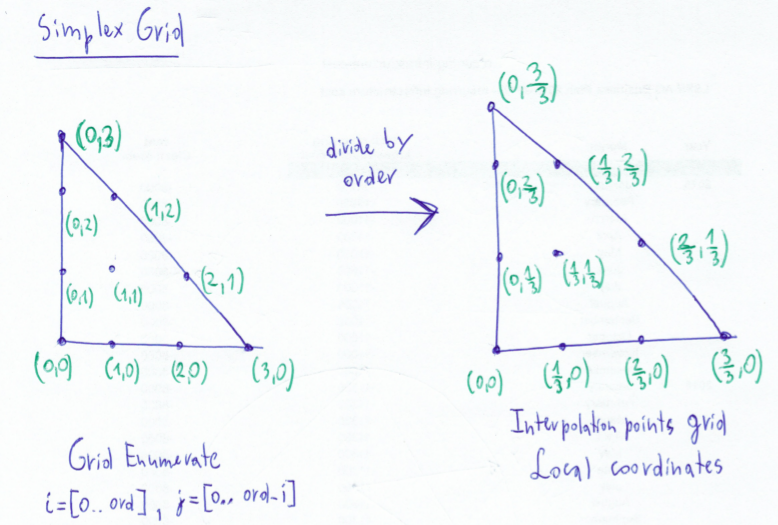
\includegraphics[scale=0.5]{doc-pics/pic-simplex-grid.png}
    %\caption{Awesome Image}
    %\label{fig:awesome_image}
\end{figure}

\noindent
After the monomials and the parametric interpolation points have been constructed, it remains to construct the interpolation matrix by evaluating the monomials at the interpolation points, then to invert the matrix, and multiply the monomial vector by it obtaining lagrange polynomials. This has been implemented both explicitly, by calculating all the lagrange interpolatory polynomials for simplices and writing them as functions, and implicitly, by introducing a polynomial class, which has all the above functionality, and thus generates a set of interpolatory polynomials which can be evaluated and integrated analytically by the code.

\subsection{Methods}

\begin{itemize}
	\item \uline{Initialization:} Requires reference element/GeometryType, interpolatory vertex vector and interpolation order
	\item \uline{dofPerOrder:} Number of interpolatory vertices required for a given element type, dimension and interpolation order. For a simplex this quantity is
	\[ {DoF}_{dim}^{ord} = \{ \{ 2,3,4,5,6 \}, \{ 3,6,10,15,21 \}, \{ 4,10,20,35,56 \} \} \]
	\item \uline{cornerID:} The id number of a corner in the interpolatory vertex vector. For the simplices is calculated as follows:
		\subitem -for edge $\{ 0, \; ord \}$
		\subitem -for triangle $\{0, \; ord, \; {DoF}_{dim}^{ord} - 1\}$
		\subitem -for tetrahedron $\{0, \; ord, \; ord (ord + 3) / 2, \; {DoF}_{dim}^{ord} - 1\}$
	\item \uline{simplexGrid:} These 3 methods implement the functionality discussed in section \ref{subsection-simplexgrid}. They return a vector of indices which the grid points take in the d-dimensional matrix, and that vector divided by the interpolation order, which is exactly the local coordinates of the reference simplex grid.
	\item \uline{lagrangePolynomial:} Evaluates the i-th Lagrange Polynomial $L_i(\vec{r})$ for a given $i$ and a given local coordinate. Lagrange polynomials in this case are given explicitly for all orders to accellerate computation.
	\item \uline{realCoordinate:} Evaluates the global coordinate given a local coordinate. Computes the scalar product $\vec{p}(\vec{r}) = \sum_i \vec{p}_i L_i (\vec{r})$.
	\item \uline{interpolatoryVectorAnalytical:} Produces an analytical map from local to global coordinates in terms of polynomial vector.
		\subitem 0) Constructs local grid points $\vec{r}_i$ as given in \ref{subsection-simplexgrid}.		
		\subitem 1) Constructs monomial basis $\vec{z}^{ord}(\vec{r})$ as given in the beginning of section \ref{section-interppoly}
		\subitem 2) Evaluates all monomials $\vec{z}^{ord}(\vec{r})$ at all local grid points $\vec{r}_i$, assembling the DynamicMatrix V
		\subitem 3) Computes all lagrange polynomials using $\vec{L}(\vec{r}) = V^{-1} \vec{z}^{ord}(\vec{r})$
		\subitem 4) Computes the analytical map $\vec{p}(\vec{r}) = \sum_i \vec{p}_i L_i (\vec{r})$.
	\item \uline{SubentityInterpolators} Constructs Interpolator classes for each $\dim - 1$ subentity of the given element. Only allowed for elements of dimensions 2 and 3.
		\subitem - At the moment a rather crude algorithm is employed. To find the vertices corresponding to a given boundary, the order numbers of simplexGrid are written in a $(ord + 1) \times (ord + 1) \times (ord + 1)$ matrix, which is then used to easier locate the indices of the boundary interpolatory points in the vertex vector.
		\subitem - Certain orientation convention is chosen for the provided sub-entitiy interpolators, to simplify the future calculation of the outwards normals. The convention for edge orientations for a triangle $(012)$ are $(01)$, $(12)$ and $(20)$. The convention for triangle orientations for a tetrahedron $(0123)$ are $(012)$, $(023)$, $(213)$ and $(031)$.
\end{itemize}

\begin{figure}[hp]
    \centering
    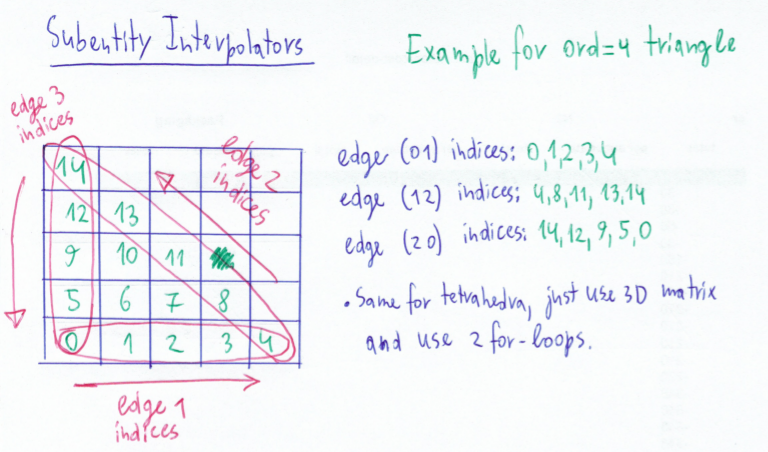
\includegraphics[scale=0.5]{doc-pics/pic-subentity-interpolators-method.png}
    %\caption{Awesome Image}
    %\label{fig:awesome_image}
\end{figure}


\subsection{Tests}

\noindent
For each dimension several linear and polynomial Functors are defined which act as pre-defined local-to-global maps. Then, for a simplex of each dimension there is a testing routine which is run for every applicable Functor. The tests are as follows:
\begin{itemize}
	\item For each order generate a local grid and sample the given functor to obtain global coordinates for interpolation points and thus construct the interpolator.
	\item First test requests a global coordinate for each local grid point, both using explicit function $realCoordinate$ and by evaluating the analytical polynomial provided by $interpolatoryVectorAnalytical$. Then the 3 results are compared. For this test, all 3 results must match independent of Functor and interpolation order.
	\item Second test requests a global coordinate for a random set of local coordinates, also comparing the correct result with explicit and analytical functionality. Explicit and analytical results should be equal to each other for any test since they do the same thing. However, they will match to the true result only if the polynomial order of the Functor is lower or equal to the one being tested, and most likely should fail for lower orders.
\end{itemize}

\textbf{TODO:}
\begin{itemize}
	\item The tests must be automatized such that the program throws an error if a test fails.
	\item Would be useful to test the method $SubentityInterpolators$ which is not tested at the moment, but is indirectly tested later in the LagrangeGeometry tests.
\end{itemize}



\section{Numerical Element Integrator class}

Evaluates integral over element, approximating the integrand by an interpolatory polymomials of two hierarchical orders (2 and 4 at the moment). The running integration error is approximated by the difference between the analytical integrals calculated from these two interpolatory polynomials. The higher order element is split into into sub-elements of lower order, and the integration proceeds recursively. Every time an element is split, its previous running error is subtracted from the total error, and the running errors of the sub-elements are added to the total error. Thus, the integration is terminated when total approximated error is below selected tolerance. Heap structure ordered by the approximate error of the element is used to avoid recursion. At every iteration the element with the worst error is selected and then refined. When splitting, the previously calculated points are not re-calculated but hierarchically re-used by sub-elements. The sub-element only needs to be refined to a higher hierarchical order, by adding more points. \\

\noindent
\textit{Possible improvement - Performance}. As the the refined element does not check if the neighboring elements are also being refined, so they both sample on the boundary twice. Does there exist a method to store/find intersection refinements faster than just compute 2nd time. Using order 4 for every new refined triangle we sample 9 new points, out of which 2 are being wasted, thus $22\%$ inefficient.

\begin{figure}[p]
    \centering
    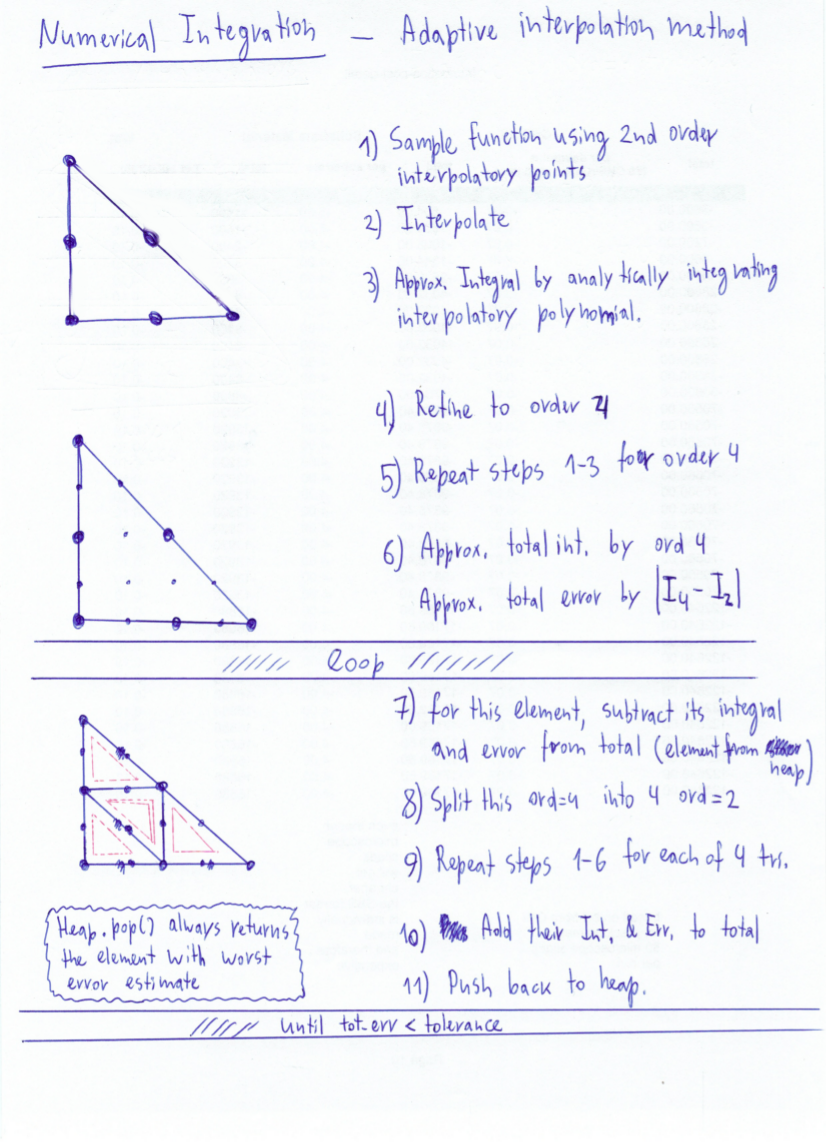
\includegraphics[scale=0.8]{doc-pics/pic-numerical-integration-adaptive-interpolation.png}
    %\caption{Awesome Image}
    %\label{fig:awesome_image}
\end{figure}


\subsection{Methods}

\noindent
Numerical Integration is only available for Simplices at the moment.

\noindent
\begin{itemize}
	\item \uline{Initialization:} Requires GeometryType to know the type of the element being integrated
	\item \uline{Integrate:} Integrates a function given by a functor object, until the expected integration error is below given tolerance.
\end{itemize}


\subsection{Tests}

\noindent
Numerical Integration is only implemented and hence tested for edges and triangles. A multitude of integrands are given in terms of Functors, starting with simple polynomial integrands and ending with integrands involving square roots of polynomials, as this is these are functions the method is expected to integrate well. The integrals are computed and compared to expected ones, which are sometimes given explicitly in numerical form, except of a lucky integral of $\iint \sqrt{xy} \; dxdy$ which happens to be $\pi / 24$. \\

\textbf{TODO:}
\begin{itemize}
	\item These tests should be automatized, which is easy to do, as they are only comparing numerical values.
	\item Integrals of complicated functions may exceed 100000 samples for this method given relative precision $10^{-5}$, which is too slow for the desired application
\end{itemize}


\newpage
\appendix

\section{Proof for polynomial summand integrals}
\noindent
Note that the series for beta-function can be written as
\[B(a+1,b+1) = \int_0^1 x^a (1-x)^b dx = \int_0^1 x^a \sum_{i=0}^b C_b^i (-1)^i x^i = \sum_{i=0}^b \frac{(-1)^i C_b^i}{a+1+i}\]

\noindent
where $C_b^i = \frac{b!}{i!(b-i)!}$ is the combinations number.

\subsection{1D}

\begin{equation}
	I_{1D} = \int_0^1 x^{\alpha} dx = \frac{x^{a + 1}}{a + 1} \biggr |_0^1 = \frac{1}{a + 1}
\end{equation}

\subsection{2D}

\begin{eqnarray*}
	I_{2D} = \int_0^1 \int_0^{1-x} x^{a} y^{b} dx dy
	& = & \frac{1}{b+1} \int_0^1 x^{a} (1-x)^{b+1} dx = \frac{1}{b+1} \beta(a + 1, b + 2) \\
	& = & \frac{1}{b+1} \frac{a!(b+1)!}{(a+b+2)!} = \frac{a!b!}{(a+b+2)!}
\end{eqnarray*}

\subsection{3D}

\begin{eqnarray*}
	I_{3D}
	& = & \int_0^1 \int_0^{1-x} \int_0^{1-x-y} x^a y^b z^c dx dy dz \\
	& = & \frac{1}{c+1} \int_0^1 \int_0^{1-x} x^a y^b (1-x-y)^{c+1} dx dy \\
	& = & \frac{1}{c+1} \int_0^1 \int_0^{1-x} x^a y^b \sum_{i=0}^{c+1} C_{c+1}^i (-1)^i y^i (1-x)^{c+1-i} dx dy \\
	& = & \sum_{i=0}^{c+1} \frac{C_{c+1}^i (-1)^i}{c+1} \int_0^1 \ x^a (1-x)^{c+1-i} \int_0^{1-x} y^{b+i} dx dy \\
	& = & \sum_{i=0}^{c+1} \frac{C_{c+1}^i (-1)^i}{(c+1)(b+1+i)} \int_0^1 \ x^a (1-x)^{c+1-i} (1-x)^{b+1+i} dx \\
	& = & \sum_{i=0}^{c+1} \frac{C_{c+1}^i (-1)^i}{(c+1)(b+1+i)} \int_0^1 \ x^a (1-x)^{b+c+2} dx \\
	& = & \sum_{i=0}^{c+1} \frac{C_{c+1}^i (-1)^i}{(c+1)(b+1+i)} \beta(a+1, b+c+3) \\
	& = & \frac{1}{c+1} \beta(b+1,c+2) \beta(a+1, b+c+3) \\
	& = & \frac{1}{c+1} \frac{b!(c+1)!}{(b+c+2)!} \frac{a! (b+c+2)!}{(a+b+c+3)!} \\
	& = &  \frac{a! b! c!}{(a+b+c+3)!}
\end{eqnarray*}





\end{document}